\documentclass[12pt]{beamer}
\usepackage{cmap}
\usepackage[T2A]{fontenc}
\usepackage[utf8]{inputenc}
\usepackage{ifluatex}
\usefonttheme[onlymath]{serif}
\usepackage{svg}
\usepackage{enumerate}
\usepackage{hyperref}
\usepackage{mathtools}
\setbeamertemplate{footline}[frame number]
\definecolor{beamer@darkgreen}{rgb}{0,0.6,0}
\setbeamercolor{normal text}{fg=black,bg=white}
\setbeamercolor{title}{fg=black,bg=beamer@darkgreen}
\setbeamercolor{frametitle}{fg=black,bg=beamer@darkgreen}
\setbeamercolor{background canvas}{parent=normal text}

\usepackage[english,russian]{babel}
\usepackage{graphicx}
\usepackage{listings}
\DeclareMathOperator{\sign}{sign}

\author{Катя Тузова}
\title{Машинное обучение}
\subtitle{Лекция 6. Метод опорных векторов.}
\date{}

\begin{document}	
\frame{\titlepage}

\begin{frame}\frametitle{Разбор летучки}
Почему линейная зависимость признаков приводит к переобучению?
\end{frame}

\begin{frame}\frametitle{Разбор летучки}
$a(\mathbf{x}, \mathbf{w}) = sign(\langle \mathbf{w}, \mathbf{x}\rangle)$\\
Линейная зависимость признаков:\\
$\forall \mathbf{x} \exists \mathbf{u}: \langle \mathbf{u}, \mathbf{x}\rangle = 0$\\
$\Rightarrow \forall \gamma: a(\mathbf{x}, \mathbf{w}) = sign(\langle \mathbf{w} + \gamma \mathbf{u}, \mathbf{x}\rangle)$\\
\vspace{5mm}
Алгоритм $a'$ работает точно также как исходный $a$.\\
А значит мы можем получить любое решение из семейства $\mathbf{w} + \gamma \mathbf{u}$
\end{frame}

\begin{frame}\frametitle{Разбор летучки}
Каким способом оценивается функция потерь при стохастическом градиенте?
\end{frame}

\begin{frame}\frametitle{Разбор летучки}
Input: $X^l$, $\alpha$, $\eta$\\
Output: $w_0, w_1, \dots, w_n$\\
\vspace{3mm}
Перемешать данные в $X^l$\\
Инициализировать: $w_j$, $j=0,\dots, n$\\
\hspace{35mm} ${Q}(\mathbf{w}) = \sum\limits_{i=1}^l \mathcal{L}(\langle \mathbf{w}, \mathbf{x_i} \rangle y_i)$\\
Повторить пока $Q$ и/или $w$ не стабилизируются:\\
\hspace{5mm} Взять $x_i$ из $X^l$\\
\hspace{5mm} Потеря: $\varepsilon_i = \mathcal{L}(\langle \mathbf{w}, \mathbf{x_i} \rangle y_i)$\\
\hspace{5mm} Градиентный шаг: $w =  w - \alpha \mathcal{L}'(\langle \mathbf{w}, \mathbf{x_i}\rangle y_i)\mathbf{x_i}y_i$\\
\hspace{5mm} Оценить $Q = (1-\eta)Q + \eta \varepsilon_i$
\end{frame}

\begin{frame}\frametitle{Разбор летучки}
Каким образом сокращаются веса при градиентном спуске? И для чего?
\end{frame}

\begin{frame}\frametitle{Разбор летучки}
Штраф за увеличение нормы вектора весов:\\
$Q_{\tau} = Q + \frac{\tau}{2}\Vert \mathbf{w} \Vert^2 \rightarrow \min\limits_{\mathbf{w}}$\\
\vspace{5mm}
Градиент:\\
$\bigtriangledown Q_{\tau} = \bigtriangledown Q + \tau \mathbf{w}$\\
\vspace{5mm}
Градиентный шаг:\\
$\mathbf{w} = \mathbf{w}(1-\alpha \tau) - \alpha \bigtriangledown Q(\mathbf{w})$\\
$\tau$ -- параметр регуляризации
\end{frame}

\begin{frame}\frametitle{Разбор летучки}
Для чего можно делать пробные случайные шаги?
\end{frame}

\begin{frame}\frametitle{Разбор летучки}
Выбивание из локальных минимумов.
\end{frame}

\begin{frame}\frametitle{Разбор летучки}
Почему возникает необходимость в изобретении метода стохастического градиента? 
\end{frame}

\begin{frame}\frametitle{Разбор летучки}
$\mathbf{w} =  \mathbf{w} - \alpha \sum\limits_{i=1}^l \mathcal{L}'(\langle \mathbf{w}, \mathbf{x_i} \rangle y_i)\mathbf{x_i}y_i$\\
\end{frame}

\begin{frame}\frametitle{Постановка задачи}
$X = \mathbb{R}^n$, ${Y = \left\{ -1, + 1\right\}}$\\
${X^l = (x_i, y_i)_{i = 1}^l}$ -- обучающая выборка\\
\vspace{5mm}Найти:\\
$(n-1)$-мерную гиперплоскость, которая разделяет данные как можно лучше.
\\ \vspace{5mm}
Как можно лучше -- это как?

\end{frame}

\begin{frame}\frametitle{Пример}
\begin{figure}[htbp]
  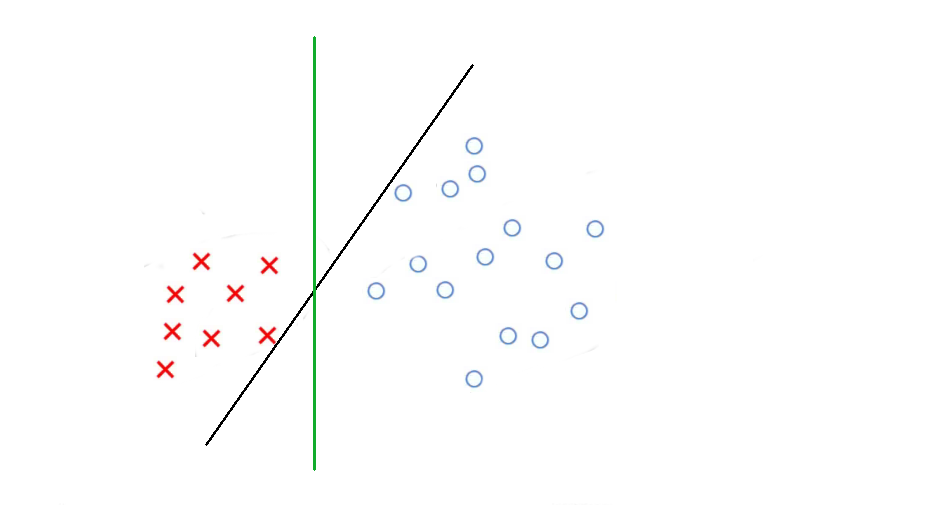
\includegraphics[height=190pt, keepaspectratio = true]{images/example}   
\end{figure}
\end{frame}

\begin{frame}\frametitle{Постановка задачи}
Как можно лучше:\\
Два разделенных класса должны лежать как можно дальше от разделяющей гиперплоскости.\\
\end{frame}

\begin{frame}\frametitle{Опорная гиперплоскость}
\end{frame}

\begin{frame}\frametitle{Опорная гиперплоскость}
Гиперплоскость называется опорной для множества точек
$X$, если все точки из $X$ лежат по одну сторону от этой гиперплоскости.\\\vspace{5mm}
${f(\mathbf{x},\mathbf{w}, w_0) = \langle \mathbf{x}, \mathbf{w}\rangle - w_0 = 0}$\\
\vspace{5mm}
Как посчитать расстояние от точки до гиперплоскости?
\end{frame}

\begin{frame}\frametitle{Опорная гиперплоскость}
Гиперплоскость называется опорной для множества точек
$X$, если все точки из $X$ лежат по одну сторону от этой гиперплоскости.\\\vspace{5mm}
${f(\mathbf{x},\mathbf{w}, w_0) = \langle \mathbf{x}, \mathbf{w}\rangle - w_0 = 0}$\\
\vspace{5mm}
Расстояние от точки до гиперплоскости:
$\frac{\vert f(\mathbf{x},\mathbf{w}, w_0) \vert}{\Vert \mathbf{w} \Vert}$
\end{frame}

\begin{frame}\frametitle{Максимизиция отступа}
Идея:\\
Максимизировать отступ между двумя параллельными опорными плоскостями, а затем провести параллельную им плоскость на равных расстояниях.\\
\end{frame}

\begin{frame}\frametitle{Постановка задачи}
${X^l = (x_i,y_i)_{i = 1}^l}$\\ 
${Y=\left\{-1,+1\right\}}$\\
\vspace{5mm}
Линейный классификатор:\\
$a(\mathbf{x}, \mathbf{w}) = sign(\langle \mathbf{w}, \mathbf{x}\rangle - w_0)$\\
\end{frame}


\begin{frame}\frametitle{Линейно разделимая выборка}
\end{frame}

\begin{frame}\frametitle{Линейно разделимая выборка}
Выборка линейно разделима, если отступ на каждом объекте положителен.\\
\vspace{5mm}
$\exists \mathbf{w}, w_0 : M_i(\mathbf{w}, w_0) = y_i  (\langle \mathbf{w}, \mathbf{x_i} \rangle - w_0) > 0$, i=1, \dots , l\\
\end{frame}

\begin{frame}\frametitle{Линейно разделимая выборка}
\begin{figure}[htbp]
  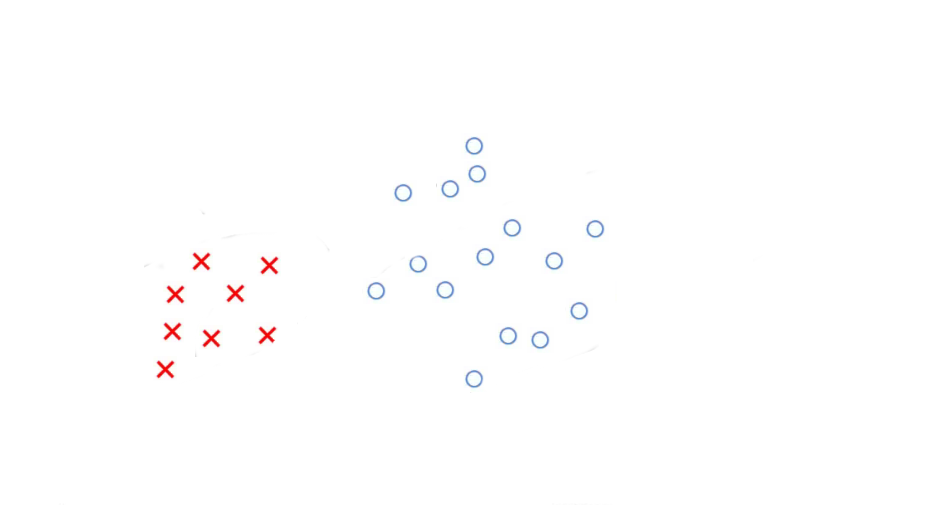
\includegraphics[height=190pt, keepaspectratio = true]{images/linearly_separable1}   
\end{figure}
\end{frame}

\begin{frame}\frametitle{Линейно неразделимая выборка}
\begin{figure}[htbp]
  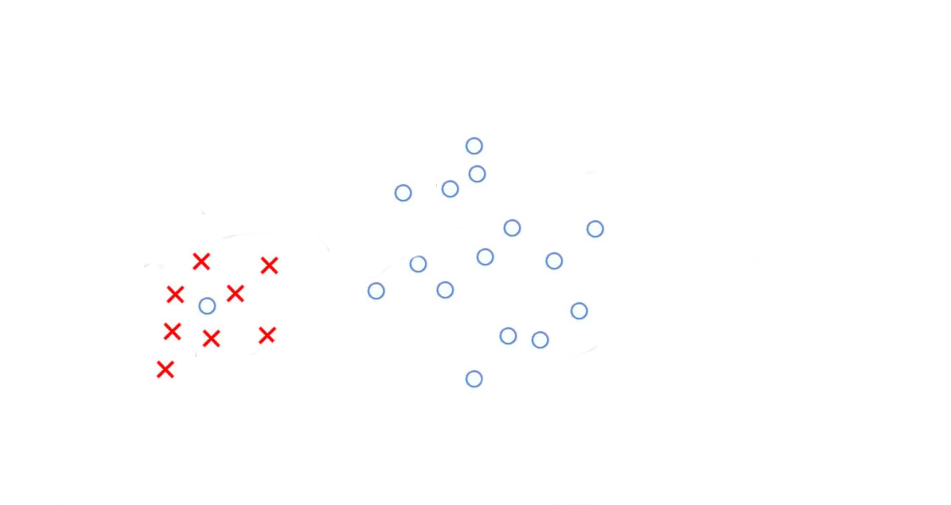
\includegraphics[height=190pt, keepaspectratio = true]{images/linearly_unseparable}   
\end{figure}
\end{frame}

\begin{frame}\frametitle{Оптимальная разделяющая гиперплоскость}
Нормировка: $\min\limits_{i = 1, \dots , l} M_i(\mathbf{w}, w_0) = 1$\\
Как выглядит разделяющая полоса?
\begin{figure}[htbp]
  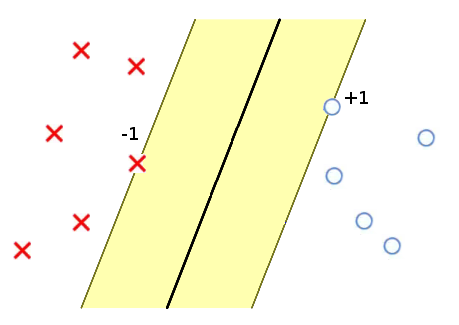
\includegraphics[height=100pt, keepaspectratio = true]{images/linearly_separable3}   
\end{figure}
\end{frame}


\begin{frame}\frametitle{Оптимальная разделяющая гиперплоскость}
Нормировка: $\min\limits_{i = 1, \dots , l} M_i(\mathbf{w}, w_0) = 1$\\
Разделяющая полоса: $\left\{\mathbf{x}: -1 \leq \langle \mathbf{w}, \mathbf{x}\rangle - w_0 \leq 1\right\}$
\begin{figure}[htbp]
  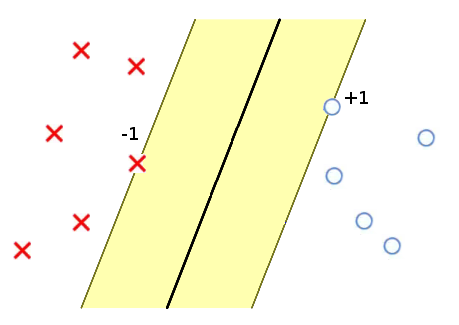
\includegraphics[height=100pt, keepaspectratio = true]{images/linearly_separable3}   
\end{figure}
\end{frame}

\begin{frame}\frametitle{Оптимальная разделяющая гиперплоскость}
Разделяющая полоса: $\left\{\mathbf{x}: -1 \leq \langle \mathbf{w}, \mathbf{x}\rangle - w_0 \leq 1\right\}$\\
Ширина разделяющей полосы?
\begin{figure}[htbp]
  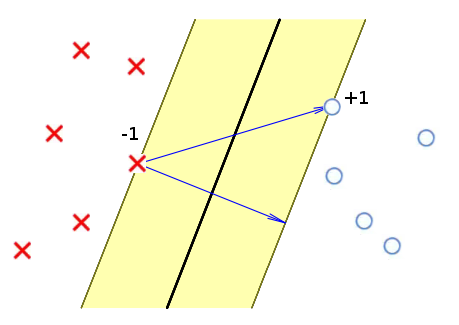
\includegraphics[height=100pt, keepaspectratio = true]{images/linearly_separable2}   
\end{figure}
\end{frame}

\begin{frame}\frametitle{Оптимальная разделяющая гиперплоскость}
Разделяющая полоса: $\left\{\mathbf{x}: -1 \leq \langle \mathbf{w}, \mathbf{x}\rangle - w_0 \leq 1\right\}$\\
Ширина разделяющей полосы: $\frac{\langle \mathbf{x_{+}}, \mathbf{w} \rangle + \langle \mathbf{x_{-}}, \mathbf{w} \rangle}{\Vert \mathbf{w} \Vert} = \frac{2}{\Vert \mathbf{w} \Vert} \rightarrow \max$\\

\begin{figure}[htbp]
  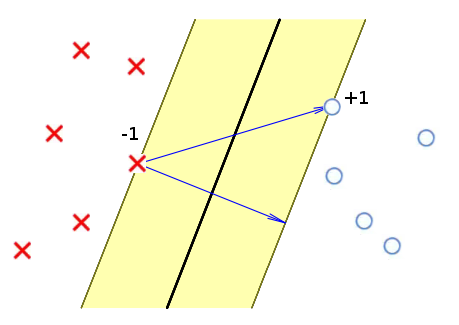
\includegraphics[height=100pt, keepaspectratio = true]{images/linearly_separable2}   
\end{figure}
\end{frame}

\begin{frame}\frametitle{Оптимальная разделяющая гиперплоскость}
Линейно разделимая выборка:\\
$\begin{cases}
{\Vert \mathbf{w} \Vert^2 \rightarrow \min\limits_{\mathbf{w}}}\\
M_i(\mathbf{w}, w_0) \geq 1
\end{cases}$\\
Линейно неразделимая выборка -- надо ослабить имеющиеся условия.\\
$\begin{cases}
{\frac{1}{2}\Vert \mathbf{w} \Vert^2 + C \sum\limits_{i=1}^l \xi_i \rightarrow \min\limits_{\mathbf{w}, \xi}}\\
M_i(\mathbf{w}, w_0) \geq 1 - \xi_i\\
\xi_i \geq 0
\end{cases}$\\
\end{frame}

\begin{frame}\frametitle{Оптимальная разделяющая гиперплоскость}
$\begin{cases}
\xi_i \geq 1 - M_i(\mathbf{w}, w_0) \\
\xi_i \geq 0
\end{cases} \Rightarrow \xi_i = 1 - M_i(\mathbf{w}, w_0) $\\
\begin{figure}[htbp]
  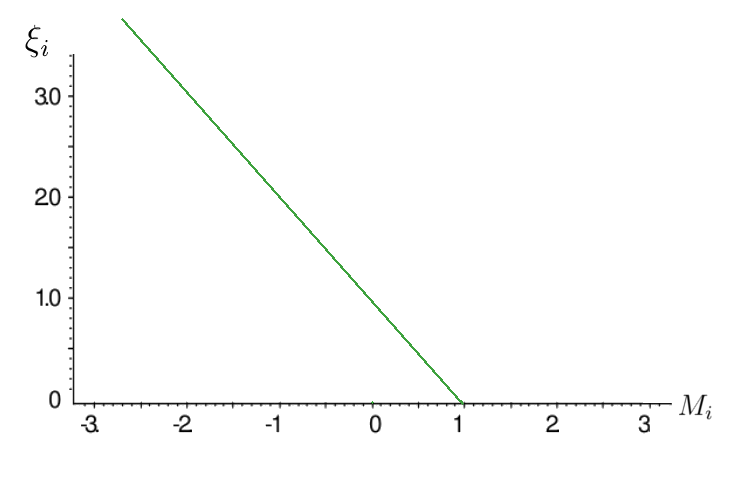
\includegraphics[height=100pt, keepaspectratio = true]{images/xi}   
\end{figure}
\end{frame}


\begin{frame}\frametitle{Задача безусловной минимизации}
$\begin{cases}
{\frac{1}{2}\Vert \mathbf{w} \Vert^2 + C \sum\limits_{i=1}^l \xi_i \rightarrow \min\limits_{\mathbf{w}, \xi}}\\
\xi_i = 1 - M_i(\mathbf{w}, w_0)
\end{cases}$\\
\vspace{5mm}
Задача безусловной минимизации:\\
$ C \sum\limits_{i=1}^l (1 - M_i(\mathbf{w}, w_0)) + \frac{1}{2}\Vert \mathbf{w} \Vert^2 \rightarrow \min\limits_{\mathbf{w}}$
\end{frame}

\begin{frame}\frametitle{Минимизация эмпирического риска}
${Q(\mathbf{w}) = \sum\limits_{i=1}^l \left[ M_i(\mathbf{w}, w_0) < 0 \right] \leq\sum\limits_{i=1}^l \mathcal{L}(M_i(\mathbf{w}, w_0)) \rightarrow \min\limits_{\mathbf{w}} }$\\\vspace{3mm}
Штраф за увеличение нормы вектора весов:\\
$Q_{\tau} = Q + \frac{\tau}{2}\Vert \mathbf{w} \Vert^2 \rightarrow \min\limits_{\mathbf{w}}$\\
\vspace{5mm}
Метод опорных векторов:\\
$ C\sum\limits_{i=1}^l (1 - M_i(\mathbf{w}, w_0)) + \frac{1}{2}\Vert \mathbf{w} \Vert^2 \rightarrow \min\limits_{\mathbf{w}}$

\end{frame}

\begin{frame}\frametitle{Примеры $\mathcal{L}$}
\begin{figure}[htbp]
  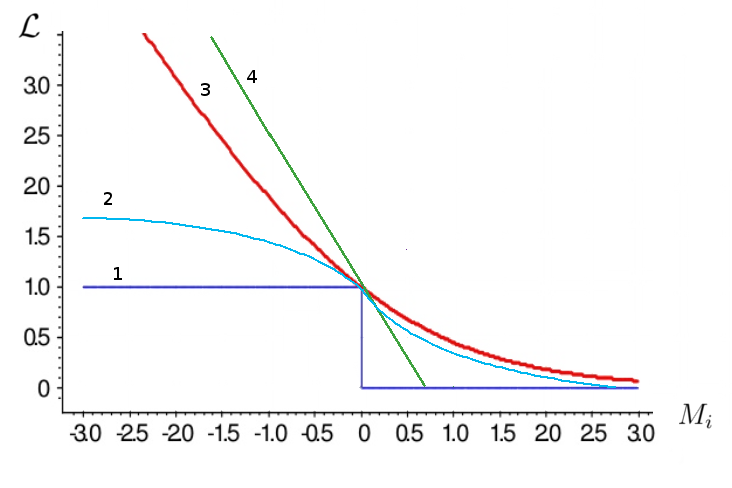
\includegraphics[height=160pt, keepaspectratio = true]{images/l}
\end{figure}
\begin{enumerate}
\item $\left[M_i(\mathbf{w}, w_0) < 0 \right]$
\item $L(M) = \log_2(1+e^{-M})$ -- логарифмическая
\item $S(M) = 2(1+e^M)^{-1}$ -- сигмоидная
\item $V(M) = (1-M)_+$ -- кусочно-линейная
\end{enumerate}
\end{frame}

\begin{frame}\frametitle{Вопрос}
$ \sum\limits_{i=1}^l (1 - M_i(\mathbf{w}, w_0)) + \frac{1}{2C}\Vert \mathbf{w} \Vert^2 \rightarrow \min\limits_{\mathbf{w}}$\\
\vspace{5mm}
На что влияет параметр $C$?
\end{frame}

\begin{frame}\frametitle{Выбор параметра $C$}
\begin{figure}[htbp]
	\begin{minipage}{.5\textwidth}
	  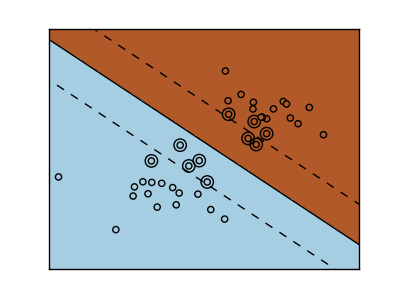
\includegraphics[height=120pt, keepaspectratio = true]{images/svm_reg} \\
		\centering Маленький $C$\\ Сильная регуляризация\\
    \end{minipage}%
    \begin{minipage}{.5\textwidth}
		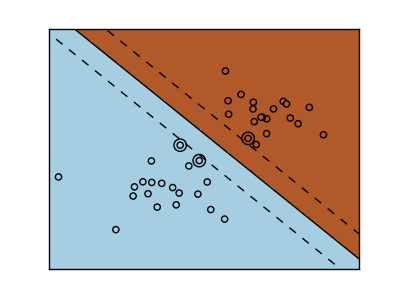
\includegraphics[height=120pt, keepaspectratio = true]{images/svm_non_reg}   \\
	  \centering Большой $C$\\ Слабая регуляризация\\
	\end{minipage}%
\end{figure}
\textcolor{gray}{Пример из Python scikit-learn: http://scikit-learn.org/dev}
\end{frame}

\begin{frame}\frametitle{Условие Каруша-Куна-Такера}
$\begin{cases}
f(x) \rightarrow \min\\
g_i(x) \leq 0 , i = 1, \dots, m\\
h_j(x) = 0 , j = 1, \dots, k\\
\end{cases}$\\
\vspace{5mm}
Двойственная задача:\\
$\begin{cases}
\mathcal{L}(x; \mu, \alpha) = f(x) + \sum\limits_{i = 1}^m \mu_ig_i(x) + \sum\limits_{j = 1}^k \alpha_jh_j(x)\\
\frac{\partial \mathcal{L}}{\partial x} = 0\\
g_i(x) \leq 0 , h_j(x) = 0\\
\mu_i \geq 0\\
\mu_ig_i(x) = 0
\end{cases}$\\

\end{frame}

\begin{frame}\frametitle{Двойственная задача SVM}
$\begin{cases}
{\frac{1}{2}\Vert \mathbf{w} \Vert^2 + C \sum\limits_{i=1}^l \xi_i \rightarrow \min\limits_{\mathbf{w}, \xi}}\\
M_i(\mathbf{w}, w_0) \geq 1 - \xi_i\\
\xi_i \geq 0
\end{cases}$\\
\vspace{5mm}
Двойственная задача:\\
$\begin{cases}
\mathcal{L} = \frac{1}{2} \Vert \mathbf{w} \Vert^2 - \sum\limits_{i = 1}^l \alpha_i (M_i(\mathbf{w}, w_0) - 1) - \sum\limits_{i = 1}^l \xi_i (\alpha_i + \mu_i - C)\\
\xi_i \geq 0,   \alpha_i \geq 0,    \mu_i \geq 0\\
\alpha_i = 0$ либо $M_i(\mathbf{w}, w_0) = 1 - \xi_i , i = 1, \dots, l\\
\mu_i = 0 $ либо $\xi_i = 0, i = 1, \dots, l
\end{cases}$
\end{frame}

\begin{frame}\frametitle{Двойственная задача SVM}
$\mathcal{L}(\mathbf{w}, w_0, \xi) = \frac{1}{2} \Vert \mathbf{w} \Vert^2 - \sum\limits_{i = 1}^l \alpha_i (M_i(\mathbf{w}, w_0) - 1) - \sum\limits_{i = 1}^l \xi_i (\alpha_i + \mu_i -C)$\\
\vspace{5mm}
$\frac{\partial \mathcal{L}}{\partial \mathbf{w}}  = \mathbf{w} - \sum\limits_{i=1}^l \alpha_iy_i\mathbf{x_i} = 0 $ \hspace{5mm} $\Rightarrow \mathbf{w} = \sum\limits_{i=1}^l \alpha_iy_i\mathbf{x_i} = 0$\\
$\frac{\partial \mathcal{L}}{\partial w_0} = - \sum\limits_{i=1}^l \alpha_iy_i = 0$ \hspace{12mm} $\Rightarrow \sum\limits_{i=1}^l \alpha_iy_i = 0$\\
$\frac{\partial \mathcal{L}}{\partial \xi_i} = -\alpha_i - \mu_i + C = 0$ \hspace{6mm}  $\Rightarrow \mu_i + \alpha_i = C$\\
\end{frame}

\begin{frame}\frametitle{Двойственная задача SVM}
$\begin{cases}
-\mathcal{L}(\alpha) = - \sum\limits_{i = 1}^l \alpha_i  + \frac{1}{2} \sum\limits_{i = 1}^l\sum\limits_{j = 1}^l \alpha_i \alpha_j y_iy_j \langle \mathbf{x_i}, \mathbf{x_j} \rangle \rightarrow \min\limits_{\alpha}\\
0 \leq \alpha_i \leq C\\
\sum\limits_{i=1}^l \alpha_iy_i = 0
\end{cases}$\\
\end{frame}

\begin{frame}\frametitle{Двойственная задача SVM}

Решение исходной задачи выражается через решение двойственной:\\
$\begin{cases}
\mathbf{w} = \sum\limits_{i = 1}^l \alpha_iy_i\mathbf{x_i}\\
w_0 = \langle \mathbf{w}, \mathbf{x_i} \rangle - y_i
\end{cases}$\\
\vspace{5mm}
Линейный классификатор:\\
$a(\mathbf{x}) = \sign(\sum\limits_{i=1}^l \alpha_iy_i \langle \mathbf{x_i}, \mathbf{x} \rangle - w_0)$

\end{frame}

\begin{frame}\frametitle{Понятие опорного вектора}
\begin{itemize}
\item[--] $\alpha_i = 0$, $M_i \geq 1$ -- неинформативные объекты
\item[--] $0 < \alpha_i < C$, $M_i = 1$ -- опорные объекты
\item[--] $\alpha_i = C$, $M_i < 1$ -- опорные объекты-нарушители
\end{itemize}

\begin{figure}[htbp]
  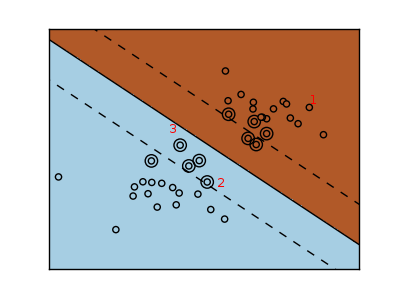
\includegraphics[height=100pt, keepaspectratio = true]{images/classification}   
\end{figure}

\end{frame}

\begin{frame}\frametitle{Двойственная задача SVM}

Решение исходной задачи выражается через решение двойственной:\\
$\begin{cases}
\mathbf{w} = \sum\limits_{i = 1}^l \alpha_iy_i\mathbf{x_i}\\
w_0 = \langle \mathbf{w}, \mathbf{x_i} \rangle - y_i
\end{cases}$\\
\vspace{5mm}
Линейный классификатор:\\
$a(\mathbf{x}) = \sign(\sum\limits_{i=1}^l \alpha_iy_i \langle \mathbf{x_i}, \mathbf{x} \rangle - w_0)$

\end{frame}

\begin{frame}\frametitle{Kernel trick}
$\langle \mathbf{x_i}, \mathbf{x} \rangle \rightarrow K(\mathbf{x_i}, \mathbf{x})$\\
\vspace{5mm}
$\psi: X \rightarrow H$, $H$ - Гильбертово пространство\\
$K(\mathbf{x_i}, \mathbf{x}) = \langle \mathbf{\psi(x_i)}, \mathbf{\psi(x)} \rangle_H$
\begin{itemize}
\item[--] $K(\mathbf{x_i}, \mathbf{x}) = K(\mathbf{x}, \mathbf{x_i})$
\item[--] неотрицательно определена
\end{itemize}
\end{frame}

\begin{frame}\frametitle{Переход к более высокой размерности}
\begin{figure}[htbp]
	\begin{minipage}{.5\textwidth}
	  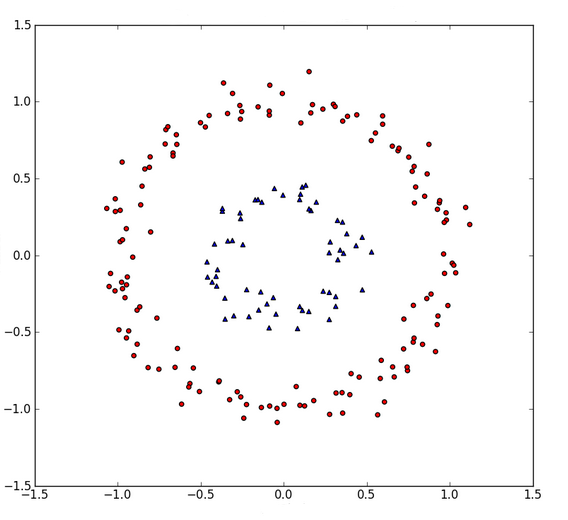
\includegraphics[height=120pt, keepaspectratio = true]{images/data-r2} \\
		\centering Данные в $\mathbb{R}^2$
    \end{minipage}%
    \begin{minipage}{.5\textwidth}
		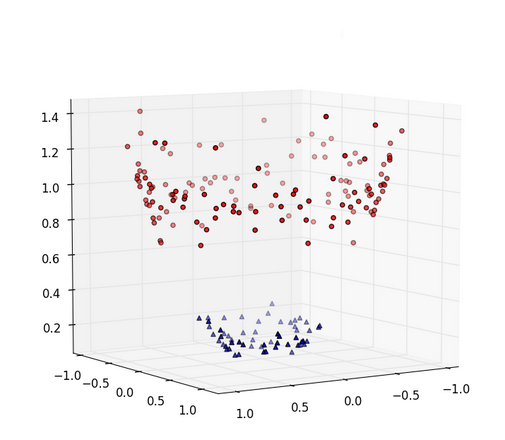
\includegraphics[height=120pt, keepaspectratio = true]{images/data-r3}   \\
		\centering Данные в $\mathbb{R}^3$
	\end{minipage}%

\end{figure}
\end{frame}

\begin{frame}\frametitle{Переход к более высокой размерности}
\begin{figure}[htbp]
	\begin{minipage}{.5\textwidth}
	  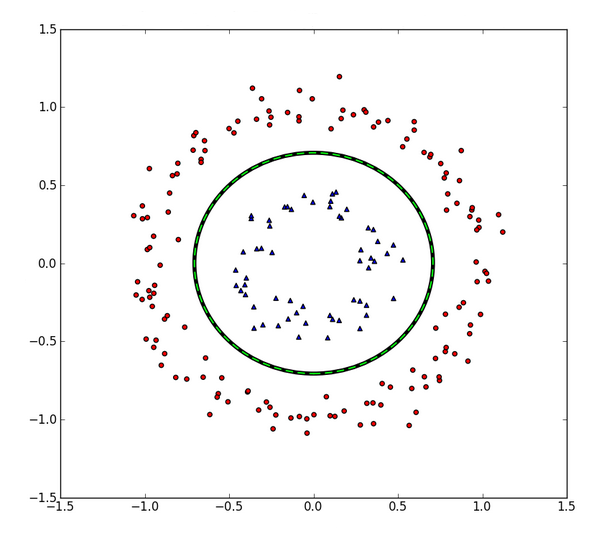
\includegraphics[height=120pt, keepaspectratio = true]{images/data-r2-1} \\
		\centering Данные в $\mathbb{R}^2$
    \end{minipage}%
    \begin{minipage}{.5\textwidth}
		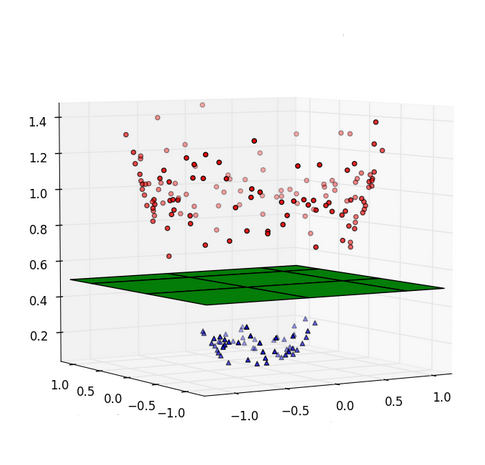
\includegraphics[height=120pt, keepaspectratio = true]{images/data-r3-1}   \\
		\centering Данные в $\mathbb{R}^3$
	\end{minipage}%

\end{figure}
\end{frame}

\begin{frame}\frametitle{Примеры ядер}
\begin{figure}[htbp]
	\begin{minipage}{.3\textwidth}
	  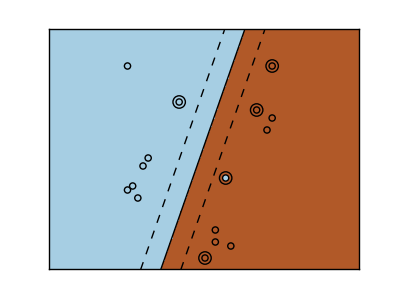
\includegraphics[height=70pt, keepaspectratio = true]{images/linear} \\
	  \centering Линейное\\$\langle x, x'\rangle$
    \end{minipage}%
    \begin{minipage}{.3\textwidth}
		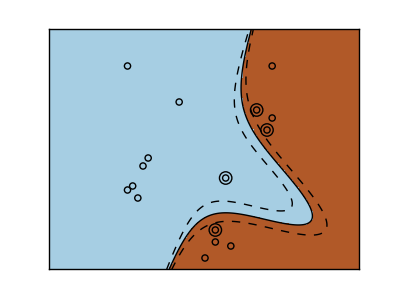
\includegraphics[height=70pt, keepaspectratio = true]{images/poly}   \\
		\centering Полиномиальное\\$(\langle x, x'\rangle + 1)^3$
	\end{minipage}%
    \begin{minipage}{.3\textwidth}
		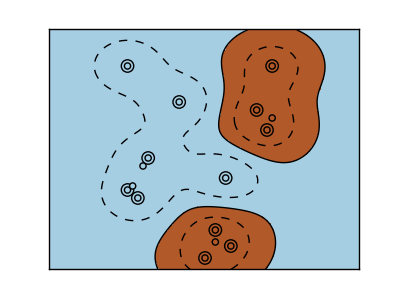
\includegraphics[height=70pt, keepaspectratio = true]{images/gauss}   \\
		\centering Гауссовское\\$exp(-\beta \Vert x - x'\Vert^2 )$
	\end{minipage}%

\end{figure}
\vspace{10mm}
\textcolor{gray}{Пример из Python scikit-learn: http://scikit-learn.org/dev}

\end{frame}

\begin{frame}\frametitle{Примеры ядер}
\begin{figure}[htbp]
  \centering Гауссовское\\$exp(-\beta \Vert x - x'\Vert^2 )$\\
  
\includegraphics[height=160pt, keepaspectratio = true]{images/svm_spiral}
\end{figure}
\end{frame}

\begin{frame}\frametitle{Конструктивные методы получения ядер}
\begin{itemize}
\item[--] $K(\mathbf{x_i}, \mathbf{x}) = \langle \mathbf{x_i}, \mathbf{x} \rangle$
\item[--] $K(\mathbf{x_i}, \mathbf{x}) = const$
\item[--] $K(\mathbf{x_i}, \mathbf{x}) = K_1(\mathbf{x_i}, \mathbf{x}) K_2(\mathbf{x_i}, \mathbf{x})$
\item[--] $K(\mathbf{x_i}, \mathbf{x}) = \alpha_1 K_1(\mathbf{x_i}, \mathbf{x}) + \alpha_2 K_2(\mathbf{x_i}, \mathbf{x})$ при  $\alpha_1, \alpha_2 > 0$
\item[--] $\forall \psi: X \rightarrow \mathbb{R}$ \hspace{5mm}$K(\mathbf{x_i}, \mathbf{x}) = \psi(\mathbf{x_i}) \psi(\mathbf{x})$
\item[--] $\forall \phi: X \rightarrow X$ \hspace{5mm}$K(\mathbf{x_i}, \mathbf{x}) = K_0(\phi(\mathbf{x_i}),  \phi(\mathbf{x}))$
\end{itemize}
\end{frame}

\begin{frame}\frametitle{Достоинства и недостатки}
\begin{itemize}
\item[+] Задача имеет единственное решение
\item[+] Число опорных векторов определяется автоматически
\end{itemize}
\begin{itemize}
\item[--] Неустойчивость к шуму
\item[--] Нет общих подходов к оптимизации ядра под задачу
\item[--] Подбор константы C
\end{itemize}
\end{frame}

\begin{frame}\frametitle{На следующей лекции}

\begin{itemize}
\item[--] Ликбез по использованию Python, Numpy, \dots
\end{itemize}
\end{frame}
\end{document}
